\section{Kết quả và quan sát}
\label{sec:results}

\noindent\fbox{\parbox{\linewidth}{\small\textbf{Ghi chú.} Số liệu ngoại tuyến
(Mục~\ref{sec:results}.1--2) lấy \emph{trực tiếp} từ lần chạy lại trên bộ dữ liệu
DongTing \emph{đầy đủ} (Zenodo 6627050; 18\,874/18\,966 chuỗi nạp được; 17/06/2026), qua quy
trình ở thư mục \texttt{Experiment/} (\texttt{results.json} + \texttt{rigorous\_metrics.json}).
Kiểm tra nhất quán đạt: AUC tập hợp mức cửa sổ tính lại $=0{,}835$ khớp
\texttt{results.json}. Báo cáo giới hạn ở \emph{đánh giá ngoại tuyến} trên DongTing
(huấn luyện $\to$ kiểm tra $\to$ đánh giá).}}

\subsection{Hiệu lực phát hiện ngoại tuyến trên DongTing}
Bảng~\ref{tab:offline} trình bày hiệu năng trên tập kiểm tra DongTing (ngưỡng chọn
trên tập kiểm định, chiến lược \texttt{p995}); Hình~\ref{fig:results} trực quan hóa. Tập kiểm tra có $687\,926$ cửa sổ
(2\,305 chuỗi); tập kiểm định $896\,581$ cửa sổ (1\,804 chuỗi).

\begin{table}[htbp]
  \centering
  \caption{Hiệu năng SyscallAD trên tập kiểm tra DongTing đầy đủ (cửa sổ $15/3$,
           43 chiều). Báo cáo ở \emph{cả} hai mức cửa sổ và chuỗi
           (Mục~\ref{subsec:protocol}); hai hàng cuối là ablation
           ``chỉ \texttt{disc}'' (Mục~\ref{subsec:confound}).}
  \label{tab:offline}
  \begin{tabular}{lccccc}
    \toprule
    \textbf{Mô hình} & \textbf{AUC} & \textbf{AP} & \textbf{F1} & \textbf{Precision} & \textbf{Recall} \\
    \midrule
    iForest (cửa sổ)            & 0{,}851 & 0{,}991 & 0{,}474 & 0{,}999 & 0{,}311 \\
    VAE (cửa sổ)                & 0{,}734 & 0{,}985 & 0{,}421 & 0{,}999 & 0{,}267 \\
    \textbf{Tập hợp (cửa sổ)}   & \textbf{0{,}835} & \textbf{0{,}990} & \textbf{0{,}417} & \textbf{0{,}999} & \textbf{0{,}264} \\
    \textbf{Tập hợp (chuỗi)}    & \textbf{0{,}787} & \textbf{0{,}871} & \textbf{0{,}502} & \textbf{0{,}977} & \textbf{0{,}338} \\
    \midrule
    Ablation chỉ \texttt{disc} (cửa sổ) & 0{,}875 & 0{,}990 & --- & --- & --- \\
    Ablation chỉ \texttt{disc} (chuỗi)  & 0{,}678 & --- & --- & --- & --- \\
    \bottomrule
  \end{tabular}

  \vspace{2pt}
  {\footnotesize VAE AUC kiểm định ổn định: $0{,}943 \pm 0{,}001$ qua 3 hạt giống
  $\{0,1,2\}$ (chọn hạt giống~1, $0{,}944$); AUC tập hợp trên tập kiểm tra
  $0{,}835 \pm 0{,}000$ qua các hạt giống.}
\end{table}

\begin{figure}[htbp]
  \centering
  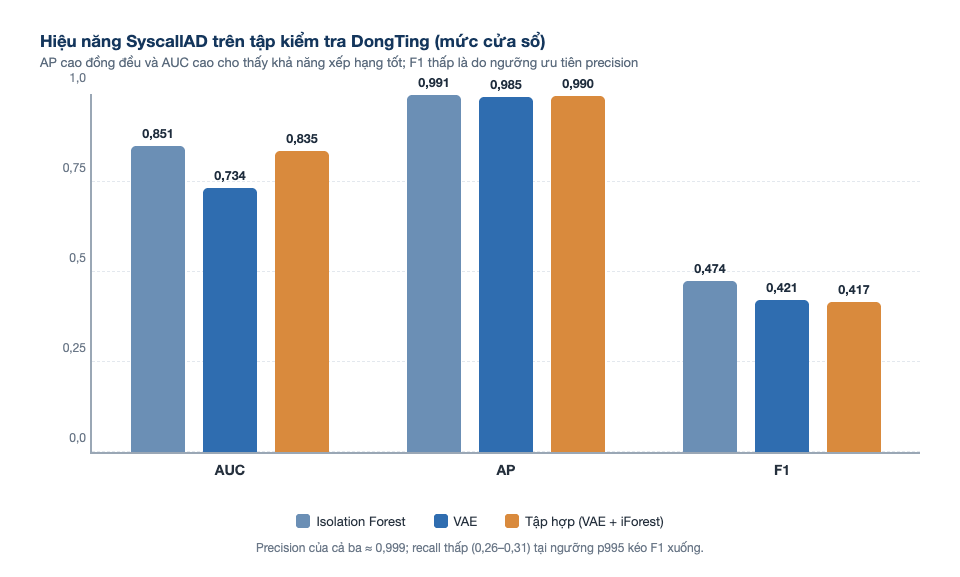
\includegraphics[width=0.92\linewidth]{figures/results-bars}
  \caption{Hiệu năng mức cửa sổ của ba mô hình trên tập kiểm tra DongTing. AP cao đồng
           đều ($\approx 0{,}99$) và AUC cao ($0{,}73$--$0{,}85$) phản ánh khả năng
           \emph{xếp hạng} tốt; F1 thấp ($0{,}42$--$0{,}47$) là hệ quả của ngưỡng
           \texttt{p995} ưu tiên precision (recall $0{,}26$--$0{,}31$).}
  \label{fig:results}
\end{figure}

\paragraph{Quan sát.} (i) \emph{Xếp hạng}: lõi phát hiện đạt AUC/AP cao và ổn định
(tập hợp AUC $0{,}835$, AP $0{,}990$; AUC tập hợp gần như bất biến qua hạt giống,
$\pm 0{,}000$). (ii) \emph{Điểm chốt nhị phân}: tại ngưỡng \texttt{p995} ưu tiên
precision ($0{,}999$), recall mức cửa sổ thấp ($0{,}264$) nên F1 thấp ($0{,}417$);
đúng như giao thức đã lường trước, chênh lệch F1 truy về \emph{chiến lược ngưỡng}
chứ không phải năng lực xếp hạng. (iii) \emph{Cửa sổ so với chuỗi}: khi gộp lên mức
chuỗi (gắn cờ nếu có cửa sổ vượt ngưỡng), recall tăng ($0{,}338$) và F1 tăng
($0{,}502$) dù AUC giảm nhẹ ($0{,}787$)---xác nhận rằng nhãn mức cửa sổ làm lệch các
chỉ số và cần báo cáo cả hai mức. (iv) \emph{Ablation}: xem
Mục~\ref{subsec:confound} (kết quả có hệ quả với phản biện cốt lõi).

\subsection{Tham chiếu định tính tới DeSFAM}
\label{subsec:qual-ref}
Một điểm cần được nêu rõ: bài báo gốc DeSFAM~\cite{desfam_original} \textbf{không
công bố bảng AUC/AP/F1 theo từng mô hình} cho SyscallAD trên DongTing. Bài chỉ nêu
vài con số \emph{tổng hợp} (precision $\approx 94\%$, recall $\approx 90\%$,
F1 $\approx 0{,}92$, AUC $\approx 0{,}94$), và những con số này thậm chí không hoàn
toàn nhất quán trong chính bài (ví dụ phần văn bản ghi F1 của riêng VAE $\approx
0{,}84$ trong khi bảng lại ghi cao hơn). Vì vậy báo cáo \emph{cố ý không} lập bảng
``đối chiếu theo mô hình với số liệu công bố''---một bảng như thế sẽ là \emph{gán
nhầm} (các phiên bản trước từng dùng các giá trị $0{,}646/0{,}747/0{,}656$ và mô tả
là ``số liệu bài báo'', đây là một sai sót đã được sửa). Ở đây chỉ tham chiếu
\emph{định tính}.

So với mức tổng hợp nói trên, bản tái lập đạt AUC/AP \emph{cùng tầm cao} (tập hợp AUC
$0{,}835$, AP $0{,}990$, precision $0{,}999$) nhưng recall/F1 \emph{thấp hơn hẳn}
($0{,}264$/$0{,}417$ mức cửa sổ). Khác biệt này quy về hai lựa chọn thiết kế đã nêu
rõ: (i) ngưỡng \texttt{p995} ưu tiên precision thay vì ngưỡng tối ưu F1 mà mức công
bố $0{,}92$ ngụ ý; (ii) bảng chữ cái 23 syscall + véc-tơ 43 chiều hẹp hơn thiết lập
đầy đủ. Báo cáo \emph{không} tuyên bố ``đạt/vượt số liệu công bố''; kết luận giới hạn
ở chỗ đã \emph{tái hiện trung thành đường ống} và giữ được khả năng xếp hạng cùng
định hướng ít báo động giả (xem tiêu chí ở Mục~\ref{subsec:protocol}).

\subsection{Cấu hình bảng chữ cái syscall an ninh}
Toàn bộ kết quả trên dùng \texttt{SENSOR\_ALPHABET=1} (lọc DongTing về đúng 23
syscall an ninh \emph{trước} khi cắt cửa sổ), cho AUC kiểm định VAE $0{,}944$. Việc
giới hạn về tập syscall an ninh là một bước \emph{chọn lọc đặc trưng theo miền}
(Mục~\ref{subsec:alphabet}), giúp bộ phát hiện tập trung vào hành vi đặc quyền. Phép
đối chứng định lượng với chế độ \texttt{SENSOR\_ALPHABET=0} (toàn bộ vũ trụ syscall)
được nêu là hướng phát triển (Mục~\ref{sec:conclusion}).
